\documentclass{article}
\usepackage[utf8]{inputenc}
\usepackage{graphicx}

\usepackage{enumerate}
\begin{document}
\section{Pregled finansijskog stanja}
Pregled finansijskog stanja je slučaj upotrebe u kojem menadžer restorana ima mogućnost pregleda prihoda i rashoda za dati vremenski period, koji se izračunavaju na osnovu naplaćenih usluga i troškova nabavke, održavanja, prihoda zaposlenih, itd.
\\
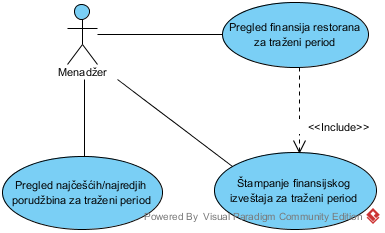
\includegraphics[width=\linewidth]{pregledFinansija.png}


\subsection{\textbf{Use Case}: Pregled finansija restorana za traženi period}
\textbf{Akter:} Menadžer\\
\textbf{Ulaz:} Datum početka perioda od interesa, datum kraja perioda od interesa\\
\textbf{Izlaz:} Tabelarni prikaz prihoda i rashoda za traženi period\\
\textbf{Preduslovi:} Menadžer ima pravo pristupa stranici za pregled finansija, svi navedeni datumi su ispravni, restoran je imao barem jedan poslovni dan u navedenom periodu.\\
\textbf{Postuslov:} Nema\\
\textbf{Glavni tok:}
\begin{enumerate}
\item Korisnik unosi korisničko ime i lozinku
\item Korisnik se prijavljuje na sistem
\item Korisnik vrši odabir početnog i krajnjeg dana perioda od interesa
\item Korisnik dobija spisak prihoda i rashoda u datom vremenskom periodu.
\end{enumerate}
\textbf{Alternativni tok:} \\
        2.1. Prijavljivanje nije uspešno, korisnik se preusmerava na poruku sa greškom.\\
        3.1. Uneti datumi nisu validni, korisnik se moli da ponovo unese datume i nastavlja na koraku 3.\\
        3.2. Za unete datume, restoran nije imao nijedan poslovni dan, prikazuje se adekvatna poruka na ekranu i korisnik se preusmerava nazad na korak 3.\\
		
\subsection{\textbf{Use Case}: Štampanje finansijskog izveštaja za traženi period}
\textbf{Akter:} Menadžer\\
\textbf{Ulaz:} Datum početka perioda od interesa, datum kraja perioda od interesa, način štampanja.\\
\textbf{Izlaz:} Tabelarni prikaz prihoda i rashoda za traženi period i .pdf verzija finansijskog izveštaja.\\
\textbf{Preduslovi:} Menadžer ima pravo pristupa stranici za pregled finansija, svi navedeni datumi su ispravni, restoran je imao barem jedan poslovni dan u navedenom periodu, postoji barem jedan štampač povezan na sistem.\\
\textbf{Postuslov:} Odštampan finansijski izveštaj ima identične podatke kao i prikazani.\\
\textbf{Glavni tok:}
\begin{enumerate}
\item Korisnik unosi korisničko ime i lozinku
\item Korisnik se prijavljuje na sistem
\item Korisnik vrši odabir početnog i krajnjeg dana perioda od interesa
\item Korisnik dobija spisak prihoda i rashoda u datom vremenskom periodu
\item Korisniku se prikazuje dijalog za štampu kreiranog izveštaja za navedeni period.
\end{enumerate}
\textbf{Alternativni tok:}\\
        2.1. Prijavljivanje nije uspešno, korisnik se preusmerava na poruku sa greškom.\\
        3.1. Uneti datumi nisu validni, korisnik se moli da ponovo unese datume i nastavlja na koraku 3.\\
        3.2. Za unete datume, restoran nije imao nijedan poslovni dan, prikazuje se adekvatna poruka na ekranu i korisnik se preusmerava nazad na korak 3.\\
        5.1 Nijedan štampač nije povezan na sistem, prikazuje se poruka o grešci.
       
\subsection{\textbf{Use Case}: Pregled najčešćih/najredjih porudžbina za traženi period.}
\textbf{Akter:} Menadžer\\
\textbf{Ulaz:} Datum početka perioda od interesa, datum kraja perioda od interesa.\\
\textbf{Izlaz:} Lista stavki sa menija koje su najčešće/najredje naručivane u traženom periodu.\\
\textbf{Preduslovi:} Menadžer ima pravo pristupa stranici za pregled finansija, svi navedeni datumi su ispravni, restoran je imao barem jedan poslovni dan u navedenom periodu.\\
\textbf{Postuslov:} Nema.\\
\textbf{Glavni tok:}
\begin{enumerate}
\item Korisnik unosi korisničko ime i lozinku
\item Korisnik se prijavljuje na sistem
\item Korisnik vrši odabir početnog i krajnjeg dana perioda od interesa
\item Korisnik dobija spisak najčešće i najredje naručivanih stavki sa menija.
\end{enumerate}
\textbf{Alternativni tok:}\\
        2.1. Prijavljivanje nije uspešno, korisnik se preusmerava na poruku sa greškom.\\
        3.1. Uneti datumi nisu validni, korisnik se moli da ponovo unese datume i nastavlja na koraku 3.\\
        3.2. Za unete datume, restoran nije imao nijedan poslovni dan, prikazuje se adekvatna poruka na ekranu i korisnik se preusmerava nazad na korak 3.\\

\end{document}
